\documentclass[11pt,a4paper]{article}
\usepackage[utf8]{inputenc}
\usepackage[vietnamese]{babel}
\usepackage{amsmath,amssymb}
\usepackage[version=4]{mhchem}
\usepackage{geometry}
\geometry{top=1.5cm,bottom=1.2cm,left=1.4cm,right=1.4cm,headheight=28pt,headsep=12pt,footskip=18pt}
\usepackage{graphicx}
\usepackage{xcolor}
\usepackage{tabularx}
\usepackage{array}
\usepackage{colortbl}
\usepackage{tikz}
\usepackage{fancyhdr}
\usepackage{enumitem}
\usepackage{multido}
\usepackage{tcolorbox}

\definecolor{hfRed}{HTML}{D32F2F}
\definecolor{hfGreen}{HTML}{8BC390}
\definecolor{mainGreen}{HTML}{2E7D32}
\definecolor{solBlue}{HTML}{1565C0}
\definecolor{tableGreen}{HTML}{E8F5E9}

\usepackage{ex_test}

\pagestyle{fancy}
\fancyhf{}
\renewcommand{\headrulewidth}{0.75pt}
\renewcommand{\headrule}{\hbox to\headwidth{\color{hfGreen}\leaders\hrule height \headrulewidth\hfill}}
\renewcommand{\footrulewidth}{0.75pt}
\renewcommand{\footrule}{\hbox to\headwidth{\color{hfGreen}\leaders\hrule height \footrulewidth\hfill}}

\fancyhead[L]{\small\itshape\color{hfRed}Tài liệu lưu hành nội bộ}
\fancyhead[R]{\small\color{hfRed}Thầy \textbf{TRẦN VĂN THẠNH} - 0777.470.803}

\fancyfoot[L]{\footnotesize\itshape\color{hfRed}CS1: 6/15 Nguyễn Hoàng, P. Kim Long, TP Huế \quad|\quad CS2: 24 Đặng Thái Thân, TP Huế}
\fancyfoot[R]{\small\textbf{\color{hfRed}Trang \thepage}}

\setlength{\parindent}{0pt}
\setlength{\parskip}{2pt}

\begin{document}

\begin{minipage}[t]{0.48\textwidth}
\textbf{SỞ GIÁO DỤC VÀ ĐÀO TẠO}\\
\textbf{TRƯỜNG THPT CAO THẮNG}\\
\textit{ĐỀ CHÍNH THỨC}\\
\textit{(Đề thi có 03 trang)}
\end{minipage}
\hfill
\begin{minipage}[t]{0.48\textwidth}
\raggedleft
\textbf{\color{hfRed}ĐỀ KIỂM TRA CUỐI KÌ 1}\\
\textbf{NĂM HỌC 2025 -- 2026}\\
\textbf{MÔN: HÓA HỌC 12}\\
\textit{Thời gian làm bài: 45 phút (không kể thời gian phát đề)}\\
\textbf{MÃ ĐỀ: 1203}
\end{minipage}

\vspace{4pt}
\noindent
\textit{Họ và tên:} \dotfill \textit{Số báo danh:} \dotfill

\vspace{3pt}
\noindent
\textit{\footnotesize Cho biết: $\ce{H}=1;\ \ce{C}=12;\ \ce{N}=14;\ \ce{Cl}=35,5;\ \ce{O}=16$.}

\vspace{3pt}
\hrule color{hfGreen} height 0.5pt

\vspace{6pt}
\begin{center}
{\Large\textbf{\color{hfRed}BẢNG ĐÁP ÁN RÚT GỌN (DÀNH CHO GIÁO VIÊN -- MÃ ĐỀ 1203)}}
\end{center}

\vspace{2pt}
\noindent
\textbf{\color{mainGreen}1. Phần I: Trắc nghiệm nhiều phương án lựa chọn (3,0 điểm)}
\begin{center}
\renewcommand{\arraystretch}{1.2}
\begin{tabular}{|c|c|c|c|c|c|c|c|c|c|c|c|c|}
\hline
\rowcolor{tableGreen}
\textbf{Câu} & \textbf{1} & \textbf{2} & \textbf{3} & \textbf{4} & \textbf{5} & \textbf{6} & \textbf{7} & \textbf{8} & \textbf{9} & \textbf{10} & \textbf{11} & \textbf{12} \\
\hline
\textbf{Đ/A} & \textbf{\color{hfRed}B} & \textbf{\color{hfRed}B} & \textbf{\color{hfRed}D} & \textbf{\color{hfRed}D} & \textbf{\color{hfRed}D} & \textbf{\color{hfRed}A} & \textbf{\color{hfRed}C} & \textbf{\color{hfRed}A} & \textbf{\color{hfRed}A} & \textbf{\color{hfRed}D} & \textbf{\color{hfRed}C} & \textbf{\color{hfRed}C} \\
\hline
\end{tabular}
\end{center}

\vspace{2pt}
\noindent
\textbf{\color{mainGreen}2. Phần II: Trắc nghiệm Đúng / Sai (2,0 điểm)}
\begin{center}
\renewcommand{\arraystretch}{1.2}
\begin{tabular}{|c|p{7.5cm}|c|c|c|c|}
\hline
\rowcolor{tableGreen}
\textbf{Câu} & \textbf{Nội dung câu hỏi} & \textbf{Lệnh a} & \textbf{Lệnh b} & \textbf{Lệnh c} & \textbf{Lệnh d} \\
\hline
\textbf{Câu 1} & Thế điện cực chuẩn \& pin điện hóa & \textbf{\color{gray}S} & \textbf{\color{hfRed}Đ} & \textbf{\color{hfRed}Đ} & \textbf{\color{gray}S} \\
\hline
\textbf{Câu 2} & Poly(vinyl chloride) (PVC) & \textbf{\color{gray}S} & \textbf{\color{hfRed}Đ} & \textbf{\color{hfRed}Đ} & \textbf{\color{gray}S} \\
\hline
\end{tabular}
\end{center}

\vspace{2pt}
\noindent
\textbf{\color{mainGreen}3. Phần III: Trắc nghiệm Trả lời ngắn (2,0 điểm)}
\begin{center}
\renewcommand{\arraystretch}{1.2}
\begin{tabular}{|c|c|c|c|c|}
\hline
\rowcolor{tableGreen}
\textbf{Câu} & \textbf{Câu 1} & \textbf{Câu 2} & \textbf{Câu 3} & \textbf{Câu 4} \\
\hline
\textbf{Đáp án} & \textbf{\color{hfRed}14,5} & \textbf{\color{hfRed}4 (hoặc 3)} & \textbf{\color{hfRed}60} & \textbf{\color{hfRed}200} \\
\hline
\end{tabular}
\end{center}

\vspace{2pt}
\noindent
\textbf{\color{mainGreen}4. Tóm tắt đáp số Phần Tự luận (3,0 điểm)}
\begin{center}
\renewcommand{\arraystretch}{1.2}
\begin{tabular}{|c|c|p{11.5cm}|}
\hline
\rowcolor{tableGreen}
\textbf{Câu} & \textbf{Điểm} & \textbf{Đáp số cốt lõi} \\
\hline
\textbf{Câu 1} & 1,0 đ & • a) $\ce{o-HOC6H4COOH + C6H5CH2OH <=> o-HOC6H4COOCH2C6H5 + H2O}$ ($\ce{H2SO4}$ đặc, $t^\circ$).\newline • b) $m(\text{ester}) = 468\text{ kg} \Rightarrow n = 2,0526\text{ kmol} \Rightarrow V(\text{benzyl alcohol}) = 266,45\text{ lít}$. \\
\hline
\textbf{Câu 2} & 1,0 đ & • a) Tơ tự nhiên: tơ tằm, len. Tơ nhân tạo: tơ visco, tơ cellulose acetate. Tơ tổng hợp: tơ nylon-6,6, tơ capron.\newline • b) Phương trình điều chế tơ nylon-6,6 và tơ capron (trùng ngưng hoặc trùng hợp mở vòng). \\
\hline
\textbf{Câu 3} & 1,0 đ & • a) Anode (cực $-$): $\ce{Cu -> Cu^2+ + 2e}$; Cathode (cực $+$): $\ce{Ag+ + 1e -> Ag}$.\newline • b) $E^\circ(\ce{Cu^2+/Cu}) = +0,34\text{ V} \Rightarrow E^\circ_{\text{pin}}(\ce{Cu-Ag}) = 0,80 - 0,34 = 0,46\text{ V}$. \\
\hline
\end{tabular}
\end{center}

\vspace{4pt}
\hrule color{hfGreen} height 0.5pt

\vspace{4pt}
\noindent
{\color{mainGreen}\textbf{\Large I. PHẦN TRẮC NGHIỆM (7,0 ĐIỂM)}}

\vspace{3pt}
\noindent
{\color{mainGreen}\textbf{\large PHẦN I. Câu trắc nghiệm nhiều phương án lựa chọn.}}\\
\textit{\small Thí sinh trả lời từ câu 1 đến câu 12. Mỗi câu hỏi thí sinh chỉ chọn một phương án.}
\vspace{2pt}

\begin{ex}
Trong pin điện hoá, quá trình khử
\choice
{không xảy ra ở cả cực âm và cực dương}
{\True xảy ra ở cực dương}
{xảy ra ở cực âm}
{xảy ra ở cực âm và cực dương}

\loigiai{
Trong pin điện hóa (Galvanic cell):\\
- Cực âm (anode): Xảy ra quá trình oxi hóa.\\
- Cực dương (cathode): Xảy ra quá trình khử (Reduction at Cathode).\\
\textbf{Chọn B.}
}
\end{ex}
\begin{ex}
Glucose là chất dinh dưỡng và được dùng làm thuốc tăng lực cho người già, trẻ em và người ốm. Số nguyên tử oxygen trong phân tử glucose là
\choice
{12}
{\True 6}
{11}
{5}

\loigiai{
Công thức phân tử của glucose là $\ce{C6H12O6}$, do đó trong một phân tử glucose có chứa 6 nguyên tử oxygen.\\
\textbf{Chọn B.}
}
\end{ex}
\begin{ex}
Quá trình cộng hợp liên tiếp nhiều phân tử nhỏ giống nhau hoặc tương tự nhau (monomer) tạo thành phân tử lớn (polymer) được gọi là phản ứng
\choice
{xà phòng hoá}
{thuỷ phân}
{trùng ngưng}
{\True trùng hợp}

\loigiai{
Theo định nghĩa: Phản ứng cộng hợp liên tiếp nhiều phân tử nhỏ giống nhau hoặc tương tự nhau tạo thành phân tử khối lớn (polymer) được gọi là phản ứng trùng hợp.\\
\textbf{Chọn D.}
}
\end{ex}
\begin{ex}
Poly(methyl methacrylate) là chất rắn trong suốt, có khả năng cho ánh sáng truyền qua tốt nên được dùng để chế tạo thuỷ tinh hữu cơ. Poly(methyl methacrylate) được điều chế từ monomer nào sau đây?
\choice
{$\ce{CH3COOC(CH3)=CH2}$}
{$\ce{CH3COOCH=CH2}$}
{$\ce{CH2=CHCOOCH3}$}
{\True $\ce{CH2=C(CH3)COOCH3}$}

\loigiai{
Poly(methyl methacrylate) (plexiglas) được trùng hợp từ monomer methyl methacrylate có công thức $\ce{CH2=C(CH3)COOCH3}$.\\
\textbf{Chọn D.}
}
\end{ex}
\begin{ex}
Polymer nào sau đây trong thành phần chỉ gồm hai nguyên tố C và H?
\choice
{Tơ nylon-6,6}
{Poly(methyl methacrylate)}
{Poly(phenol formaldehyde)}
{\True Polybuta-1,3-diene}

\loigiai{
- Tơ nylon-6,6: $\ce{[-NH-(CH2)6-NH-CO-(CH2)4-CO-]_n}$ chứa C, H, N, O.\\
- Poly(methyl methacrylate): $\ce{[-CH2-C(CH3)(COOCH3)-]_n}$ chứa C, H, O.\\
- Poly(phenol formaldehyde): chứa C, H, O.\\
- Polybuta-1,3-diene: $\ce{[-CH2-CH=CH-CH2-]_n}$ là hydrocarbon polymer chỉ gồm hai nguyên tố C và H.\\
\textbf{Chọn D.}
}
\end{ex}
\begin{ex}
Phát biểu nào sau đây là bản chất của sự lưu hoá cao su?
\choice
{\True Tạo cầu nối disulfide giữa các mạch phân tử cao su}
{Tạo loại cao su nhẹ hơn}
{Giảm giá thành cao su}
{Làm cao su dễ ăn khuôn}

\loigiai{
Bản chất của sự lưu hóa cao su là việc tạo ra các cầu nối disulfide ($\ce{-S-S-}$) nối các mạch polymer cao su riêng lẻ thành mạng không gian 3 chiều, giúp cao su đàn hồi hơn, chịu nhiệt, mài mòn tốt hơn.\\
\textbf{Chọn A.}
}
\end{ex}
\begin{ex}
Trong các chất sau, chất nào là amin bậc II?
\choice
{$\ce{CH3-CH(CH3)-NH2}$}
{$\ce{C6H5NH2}$}
{\True $\ce{CH3-NH-CH3}$}
{$\ce{H2N-[CH2]6-NH2}$}

\loigiai{
Bậc của amine bằng số nguyên tử H trong phân tử $\ce{NH3}$ bị thay thế bởi gốc hydrocarbon. $\ce{CH3-NH-CH3}$ (dimethylamine) có 2 gốc methyl gắn vào nguyên tử N nên là amine bậc II.\\
\textbf{Chọn C.}
}
\end{ex}
\begin{ex}
Ở điều kiện chuẩn, thiết lập được điện cực zinc ($\ce{Zn}$) bằng cách nhúng thanh $\ce{Zn}$ vào dung dịch
\choice
{\True $\ce{ZnSO4}\ 1\text{ M}$}
{$\ce{H2SO4}\ 1\text{ M}$}
{$\ce{NaCl}\ 1\text{ M}$}
{$\ce{HCl}\ 1\text{ M}$}

\loigiai{
Điện cực chuẩn zinc ($\ce{Zn^2+/Zn}$) được thiết lập bằng cách nhúng thanh kim loại $\ce{Zn}$ vào dung dịch chứa ion $\ce{Zn^2+}$ nồng độ $1\text{ M}$ (ví dụ $\ce{ZnSO4}\ 1\text{ M}$) ở điều kiện chuẩn ($25\ ^\circ\text{C}, 1\text{ bar}$).\\
\textbf{Chọn A.}
}
\end{ex}
\begin{ex}
Trùng hợp propylene thu được polymer có tên gọi là
\choice
{\True polypropylene}
{polyethylene}
{polystyrene}
{poly(vinyl chloride)}

\loigiai{
Trùng hợp propylene ($\ce{CH2=CH-CH3}$) thu được polymer tương ứng là polypropylene (PP).\\
\textbf{Chọn A.}
}
\end{ex}
\begin{ex}
Chất nào sau đây thuộc loại $\alpha$-amino acid?
\choice
{$\ce{H2NCH2CH2COOH}$}
{$\ce{HOCH2COOH}$}
{$\ce{H2NCH(CH3)NH2}$}
{\True $\ce{H2NCH(CH3)COOH}$}

\loigiai{
$\alpha$-amino acid là amino acid có nhóm $-\ce{NH2}$ gắn vào nguyên tử carbon số 2 (ngay kề nhóm $-\ce{COOH}$). $\ce{H2NCH(CH3)COOH}$ (alanine) là một $\alpha$-amino acid.\\
\textbf{Chọn D.}
}
\end{ex}
\begin{ex}
Chất hữu cơ $\ce{X}$ có nhiều trong cây mía, hoa thốt nốt, củ cải đường,... Nồng độ của $\ce{X}$ trong nước mía có thể đạt tới 13\%. Chất $\ce{X}$ là
\choice
{fructose}
{maltose}
{\True saccharose}
{glucose}

\loigiai{
Saccharose (sucrose) là chất kết tinh có nhiều trong cây mía, củ cải đường và hoa thốt nốt.\\
\textbf{Chọn C.}
}
\end{ex}
\begin{ex}
Phát biểu nào sau đây không đúng?
\choice
{Tơ nylon-6,6 được điều chế bằng phản ứng trùng ngưng}
{Tơ nitron được điều chế bằng phản ứng trùng hợp}
{\True Tơ tằm thuộc loại tơ bán tổng hợp}
{Cao su lưu hóa có cấu trúc mạng không gian}

\loigiai{
Tơ tằm là tơ thiên nhiên (protein thiên nhiên từ kén tằm), không phải tơ bán tổng hợp (tơ bán tổng hợp là tơ visco, tơ cellulose acetate).\\
\textbf{Chọn C.}
}
\end{ex}
\vspace{4pt}
\noindent
{\color{mainGreen}\textbf{\large PHẦN II. Câu trắc nghiệm đúng sai.}}\\
\textit{\small Thí sinh trả lời từ câu 1 đến câu 2. Trong mỗi ý a), b), c), d) ở mỗi câu, thí sinh chọn đúng hoặc sai.}
\vspace{2pt}

\begin{ex}
Cho các cặp oxi hóa - khử và thế điện cực chuẩn sau:
\begin{center}
\renewcommand{\arraystretch}{1.2}
\begin{tabular}{|c|c|c|c|c|c|}
\hline
\rowcolor{tableGreen}
\textbf{Cặp oxi hóa-khử} & $\ce{Zn^2+/Zn}$ & $\ce{Cu^2+/Cu}$ & $\ce{Fe^2+/Fe}$ & $\ce{Pb^2+/Pb}$ & $\ce{Fe^3+/Fe^2+}$ \\
\hline
$E^\circ\ (\text{V})$ & $-0,76$ & $0,34$ & $-0,44$ & $-0,13$ & $0,77$ \\
\hline
\end{tabular}
\end{center}
\choiceTF
{Cho $\ce{Zn}$ dư tác dụng với dung dịch $\ce{FeCl3}$ đến khi phản ứng hoàn toàn thu được dung dịch gồm $\ce{FeCl2}$ và $\ce{ZnCl2}$}
{\True Tính oxi hoá của $\ce{Fe^3+} > \ce{Cu^2+} > \ce{Pb^2+} > \ce{Fe^2+} > \ce{Zn^2+}$}
{\True Sức điện động chuẩn của pin $\ce{Fe-Cu}$ có giá trị là $0,78\text{ V}$}
{Cho kim loại $\ce{Fe}$ tác dụng với dung dịch $\ce{Cu(NO3)2}$ dư, đến khi phản ứng xảy ra hoàn toàn, thu được dung dịch gồm $\ce{Cu(NO3)2}$ và $\ce{Fe(NO3)3}$}

\loigiai{
a) \textbf{Sai}: Vì kim loại $\ce{Zn}$ dùng dư nên $\ce{Zn}$ sẽ khử hết $\ce{Fe^3+}$ về $\ce{Fe^2+}$ ($\ce{Zn + 2Fe^3+ -> Zn^2+ + 2Fe^2+}$), sau đó $\ce{Zn}$ dư tiếp tục khử $\ce{Fe^2+}$ về kim loại $\ce{Fe}$ ($\ce{Zn + Fe^2+ -> Zn^2+ + Fe\downarrow}$). Do đó dung dịch sau cùng chỉ chứa $\ce{ZnCl2}$, không còn $\ce{FeCl2}$.\\
b) \textbf{Đúng}: Căn cứ theo giá trị thế điện cực chuẩn: thế điện cực chuẩn càng lớn thì dạng oxi hóa có tính oxi hóa càng mạnh: $E^\circ(\ce{Fe^3+/Fe^2+}) = 0,77\text{ V} > E^\circ(\ce{Cu^2+/Cu}) = 0,34\text{ V} > E^\circ(\ce{Pb^2+/Pb}) = -0,13\text{ V} > E^\circ(\ce{Fe^2+/Fe}) = -0,44\text{ V} > E^\circ(\ce{Zn^2+/Zn}) = -0,76\text{ V}$. Vậy tính oxi hóa: $\ce{Fe^3+} > \ce{Cu^2+} > \ce{Pb^2+} > \ce{Fe^2+} > \ce{Zn^2+}$.\\
c) \textbf{Đúng}: $E^\circ_{\text{pin}}(\ce{Fe-Cu}) = E^\circ(\text{cathode}) - E^\circ(\text{anode}) = E^\circ(\ce{Cu^2+/Cu}) - E^\circ(\ce{Fe^2+/Fe}) = 0,34 - (-0,44) = 0,78\text{ V}$.\\
d) \textbf{Sai}: Phản ứng giữa $\ce{Fe}$ và $\ce{Cu(NO3)2}$: $\ce{Fe + Cu^2+ -> Fe^2+ + Cu\downarrow}$. Do $E^\circ(\ce{Fe^3+/Fe^2+}) = 0,77\text{ V} > E^\circ(\ce{Cu^2+/Cu}) = 0,34\text{ V}$ nên ion $\ce{Cu^2+}$ không thể oxi hóa tiếp $\ce{Fe^2+}$ lên $\ce{Fe^3+}$. Dung dịch thu được gồm $\ce{Cu(NO3)2}$ dư và $\ce{Fe(NO3)2}$ (không tạo $\ce{Fe(NO3)3}$).
}
\end{ex}
\begin{ex}
Poly(vinyl chloride) (PVC) là chất dẻo có tính cách điện tốt, bền với acid, dùng phổ biến để sản xuất vật liệu cách điện, ống dẫn nước, áo mưa.
\begin{center}
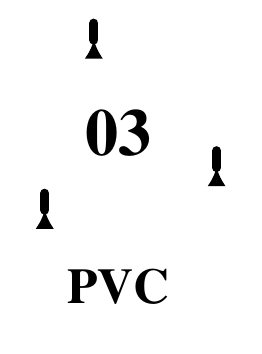
\includegraphics[width=2.0cm]{San_Pham/images_de1203/pvc_logo.png}
\end{center}
\choiceTF
{Poly(vinyl chloride) được điều chế từ vinyl chloride bằng phản ứng trùng ngưng}
{\True Cho sơ đồ chuyển hóa: $\ce{CH4 -> C2H2 -> C2H3Cl -> PVC}$. Để tổng hợp $250\text{ kg}$ PVC theo sơ đồ trên thì cần $396,64\text{ m}^3$ khí $\ce{CH4}$ (hiệu suất của cả quá trình là $50\%$)}
{\True Công thức của vinyl chloride là $\ce{CH2=CHCl}$}
{X kém bền với acid}

\loigiai{
a) \textbf{Sai}: Poly(vinyl chloride) được điều chế từ monomer vinyl chloride bằng phản ứng TRÙNG HỢP (nhờ liên kết đôi $\ce{C=C}$), không phải phản ứng trùng ngưng: $n\ce{CH2=CH-Cl -> [-CH2-CH(Cl)-]_n}$.\\
b) \textbf{Đúng}: Sơ đồ: $2\ce{CH4 -> C2H2 -> C2H3Cl -> 1/n [-C2H3Cl-]_n}$.\\
Khối lượng mol của 1 mắt xích PVC là $M = 62,5\text{ g/mol}$.\\
Số mol mắt xích PVC: $n = 250 / 62,5 = 4\text{ kmol}$.\\
Số mol $\ce{CH4}$ theo lí thuyết: $n_{\text{lt}} = 2 \times 4 = 8\text{ kmol}$.\\
Vì hiệu suất $H = 50\%$ nên số mol $\ce{CH4}$ thực tế cần: $n_{\text{tt}} = 8 / 0,5 = 16\text{ kmol}$.\\
Thể tích khí $\ce{CH4}$ ở đkc ($25\ ^\circ\text{C}, 1\text{ bar}$ với $V_{\text{mol}} = 24,79\text{ L/mol}$): $V = 16 \times 24,79 = 396,64\text{ m}^3$.\\
c) \textbf{Đúng}: Vinyl chloride là dẫn xuất monochloro của ethylene có công thức cấu tạo là $\ce{CH2=CHCl}$.\\
d) \textbf{Sai}: Đề bài đã khẳng định ngay trong đoạn dẫn: ``Poly(vinyl chloride) (PVC) là chất dẻo có tính cách điện tốt, bền với acid...'', nên phát biểu X kém bền với acid là sai.
}
\end{ex}
\vspace{4pt}
\noindent
{\color{mainGreen}\textbf{\large PHẦN III. Câu trắc nghiệm trả lời ngắn.}}\\
\textit{\small Thí sinh trả lời từ câu 1 đến câu 4. Thí sinh điền kết quả vào ô trả lời tương ứng.}
\vspace{2pt}

\begin{ex}
Caprolactam được tổng hợp từ cuối thế kỉ XIX. Hiện nay, nhu cầu sản xuất caprolactam trên thế giới khoảng 10 triệu tấn/năm. 90\% trong đó dùng để tổng hợp tơ capron. Trong công nghiệp, caprolactam được điều chế theo sơ đồ sau:
\begin{center}
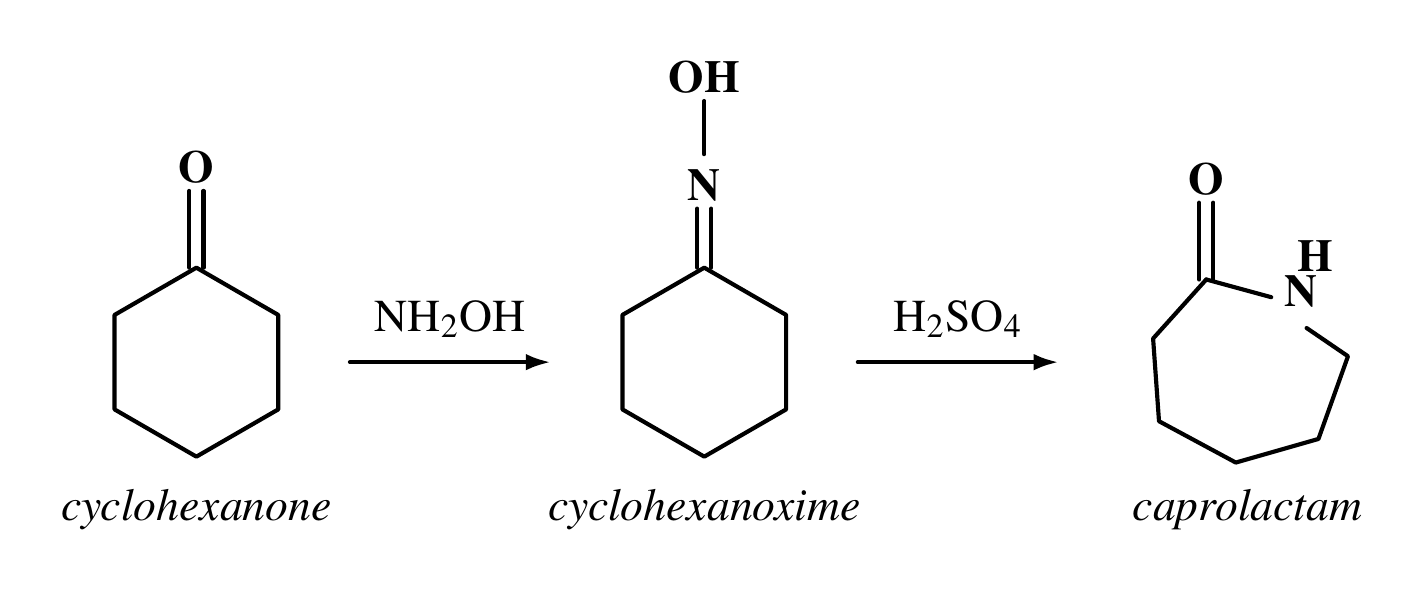
\includegraphics[width=13.5cm]{San_Pham/images_de1203/so_do_caprolactam.png}
\end{center}
Để sản xuất 10 triệu tấn caprolactam, cần sử dụng bao nhiêu triệu tấn cyclohexanone? Giả sử hiệu suất trung bình của cả quá trình trên là $60\%$. \textit{(Kết quả làm tròn đến hàng phần mười)}.
\hfill \textbf{Trả lời:} \dotfill

\loigiai{
- Khối lượng mol của Cyclohexanone ($\ce{C6H10O}$): $M = 98\text{ g/mol}$.\\
- Khối lượng mol của Caprolactam ($\ce{C6H11NO}$): $M = 113\text{ g/mol}$.\\
Sơ đồ bảo toàn: $\ce{C6H10O -> C6H11NO}$.\\
Cứ $98\text{ tấn}$ cyclohexanone tạo $113\text{ tấn}$ caprolactam theo lí thuyết.\\
Khối lượng cyclohexanone theo lí thuyết cần để sản xuất $10\text{ triệu tấn}$ caprolactam:\\
$m_{\text{lt}} = \dfrac{10 \times 98}{113} \approx 8,672566\text{ triệu tấn}$.\\
Vì hiệu suất trung bình $H = 60\% = 0,6$ nên khối lượng cyclohexanone thực tế cần dùng là:\\
$m_{\text{tt}} = \dfrac{m_{\text{lt}}}{0,6} = \dfrac{10 \times 98}{113 \times 0,6} = \dfrac{980}{67,8} \approx 14,45428\text{ triệu tấn}$.\\
Làm tròn đến hàng phần mười: \textbf{14,5}.\\
\textbf{Đáp án: 14,5}
}
\end{ex}
\begin{ex}
Cho các nguyên liệu: dầu mỏ, acid béo, dầu thực vật, sodium hydroxide, sulfuric acid, mỡ động vật. Có bao nhiêu chất sử dụng được để điều chế xà phòng trực tiếp bằng phản ứng xà phòng hóa?
\hfill \textbf{Trả lời:} \dotfill

\loigiai{
Phản ứng xà phòng hóa là phản ứng thủy phân chất béo trong dung dịch kiềm (hoặc trung hòa acid béo bằng dung dịch kiềm) để điều chế xà phòng.\\
- Dầu thực vật và mỡ động vật: Chứa triglyceride (chất béo) phản ứng trực tiếp với kiềm tạo xà phòng.\\
- Acid béo: Tác dụng trực tiếp với kiềm theo phản ứng xà phòng hóa (trung hòa) tạo muối acid béo (xà phòng).\\
- Sodium hydroxide ($\ce{NaOH}$): Là chất kiềm bắt buộc tham gia trực tiếp vào phản ứng xà phòng hóa.\\
(Dầu mỏ dùng sản xuất chất giặt rửa tổng hợp; $\ce{H2SO4}$ là xúc tác thủy phân acid).\\
Do đó, có \textbf{4} chất (hoặc 3 chất nếu chỉ tính nguyên liệu hữu cơ tạo muối xà phòng).\\
\textbf{Đáp án: 4 (hoặc 3)}
}
\end{ex}
\begin{ex}
Cho sơ đồ chuyển hóa sau (mỗi mũi tên là một phản ứng):\\
$\text{Tinh bột} \longrightarrow \ce{X} \longrightarrow \ce{Y} \longrightarrow \ce{Z} \longrightarrow \text{methyl acetate}$. Xác định phân tử khối của $\ce{Z}$.
\hfill \textbf{Trả lời:} \dotfill

\loigiai{
- Thủy phân tinh bột: $\ce{[-C6H10O5-]_n + n H2O -> n C6H12O6}$ (Glucose, $\ce{X}$).\\
- Lên men rượu: $\ce{C6H12O6 -> 2 C2H5OH + 2 CO2}$ (Ethanol, $\ce{Y}$).\\
- Lên men giấm: $\ce{C2H5OH + O2 -> CH3COOH + H2O}$ (Acetic acid, $\ce{Z}$).\\
- Este hóa: $\ce{CH3COOH + CH3OH <=> CH3COOCH3 + H2O}$.\\
Vậy chất $\ce{Z}$ là acetic acid ($\ce{CH3COOH}$).\\
Phân tử khối của $\ce{Z}$: $M(\ce{CH3COOH}) = 12 \times 2 + 4 \times 1 + 16 \times 2 = 60\text{ amu}$.\\
\textbf{Đáp án: 60}
}
\end{ex}
\begin{ex}
Khi thuỷ phân hoàn toàn $500\text{ gam}$ protein $\ce{X}$ thì thu được $178\text{ gam}$ alanine. Nếu phân tử khối của $\ce{X}$ là $50000$ thì số mắt xích alanine trong phân tử $\ce{X}$ là bao nhiêu?
\hfill \textbf{Trả lời:} \dotfill

\loigiai{
Khối lượng mol của alanine ($\ce{C3H7NO2}$): $M = 89\text{ g/mol}$.\\
Số mol alanine thu được: $n(\text{Ala}) = 178 / 89 = 2,0\text{ mol}$.\\
Số mol phân tử protein $\ce{X}$: $n(\ce{X}) = 500 / 50000 = 0,01\text{ mol}$.\\
Số mắt xích alanine trong một phân tử protein $\ce{X}$:\\
$k = \dfrac{n(\text{Ala})}{n(\ce{X})} = \dfrac{2,0}{0,01} = 200$.\\
\textbf{Đáp án: 200}
}
\end{ex}
\vspace{4pt}
\noindent
{\color{mainGreen}\textbf{\Large II. PHẦN TỰ LUẬN (3,0 ĐIỂM)}}

\vspace{3pt}

\noindent
\textbf{Câu 1. (1,0 điểm)} Benzyl salicylate được sử dụng làm chất cố định hương nước hoa, các sản phẩm khử mùi, kem chống nắng... Chất này được điều chế bằng phản ứng giữa salicylic acid ($o$-hydroxy benzoic acid) và benzyl alcohol.\\
a. Viết phương trình hoá học của các phản ứng điều chế ester trên.\\
b. Để sản xuất $400\text{ lít}$ benzyl salicylate nguyên chất ($D = 1,17\text{ g/mL}$) thì cần tối thiểu bao nhiêu lít benzyl alcohol nguyên chất ($D = 1,04\text{ g/mL}$), biết hiệu suất phản ứng là $80\%$.

\begin{center}
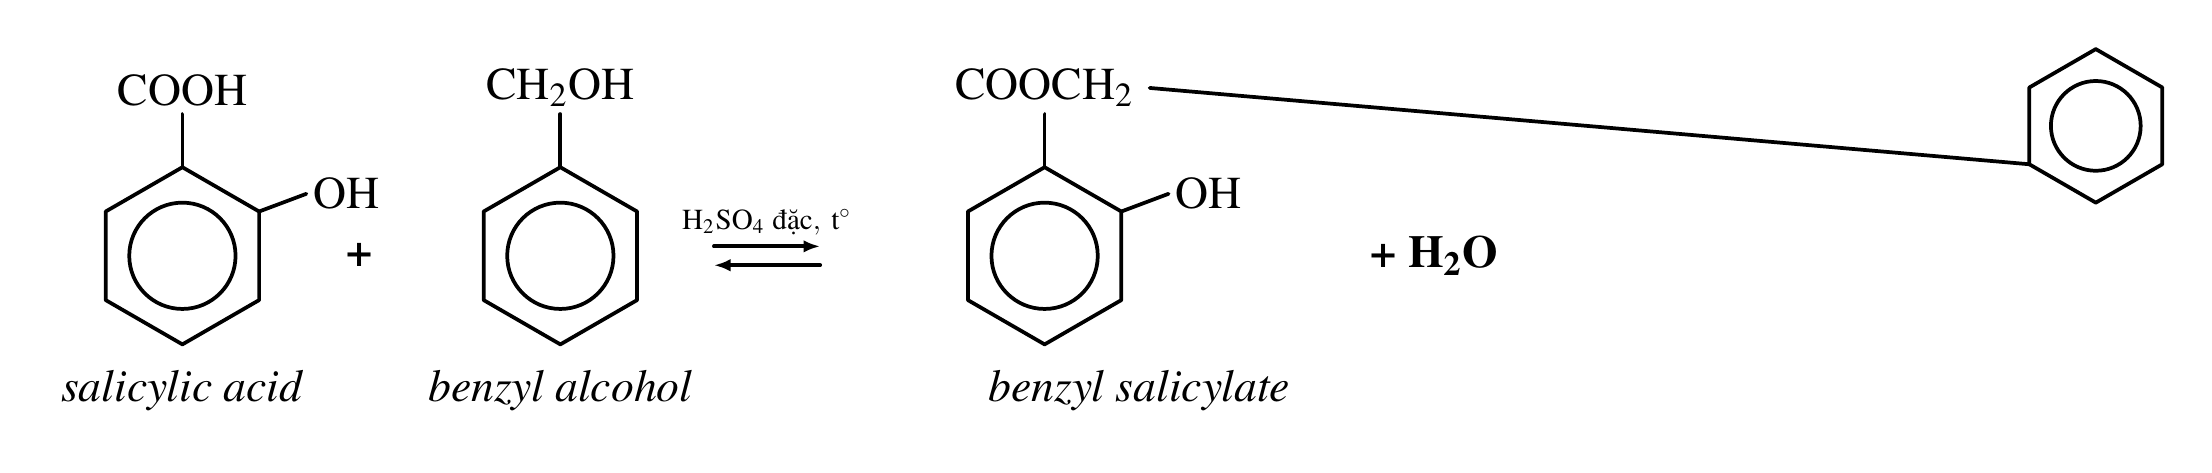
\includegraphics[width=13.5cm]{San_Pham/images_de1203/benzyl_salicylate.png}
\end{center}
\begin{tcolorbox}[colback=tableGreen!30,colframe=mainGreen!70,title=\textbf{Hướng dẫn giải chi tiết Câu 1},fonttitle=\bfseries]
\textbf{a. Phương trình hóa học điều chế ester:}\\
Nhóm $-\ce{OH}$ phenol không phản ứng este hóa trực tiếp với alcohol thông thường. Chỉ có nhóm carboxyl $-\ce{COOH}$ của salicylic acid phản ứng este hóa với benzyl alcohol:\\
\ce{o-HO-C6H4-COOH + C6H5CH2OH <=> o-HO-C6H4-COOCH2C6H5 + H2O}\quad ($\ce{H2SO4}$ đặc, $t^\circ$)\\[4pt]
\textbf{b. Tính thể tích benzyl alcohol cần dùng:}\\
1. Khối lượng benzyl salicylate cần sản xuất: $m(\text{ester}) = 400 \times 1,17 = 468\text{ kg}$.\\
2. Phân tử khối của benzyl salicylate ($\ce{C14H12O3}$): $M = 228\text{ g/mol}$.\\
$\Rightarrow n(\text{ester}) = \dfrac{468}{228} = \dfrac{39}{19} \approx 2,05263\text{ kmol}$.\\
3. Vì hiệu suất phản ứng $H = 80\% = 0,8$ nên số mol benzyl alcohol cần dùng:\\
$n(\text{alcohol}) = \dfrac{n(\text{ester})}{0,8} = \dfrac{39}{19 \times 0,8} = \dfrac{39}{15,2} \approx 2,56579\text{ kmol}$.\\
4. Khối lượng benzyl alcohol thực tế cần dùng ($M = 108\text{ g/mol}$):\\
$m(\text{alcohol}) = 2,56579 \times 108 \approx 277,1053\text{ kg}$.\\
5. Thể tích benzyl alcohol nguyên chất cần dùng ($D = 1,04\text{ kg/lít}$):\\
$V(\text{alcohol}) = \dfrac{m}{D} = \dfrac{277,1053}{1,04} \approx \mathbf{266,45\text{ lít}}$.
\end{tcolorbox}

\vspace{4pt}
\noindent
\textbf{Câu 2. (1,0 điểm)} Trong số các loại tơ sau: tơ tằm, tơ visco, tơ nylon-6,6, len, tơ cellulose acetate, tơ capron.\\
a. Tơ nào là tơ tự nhiên, tơ nhân tạo và tơ tổng hợp?\\
b. Viết phương trình hoá học của phản ứng điều chế các loại tơ tổng hợp ở trên từ các monomer tương ứng (ghi rõ điều kiện nếu có).

\begin{tcolorbox}[colback=tableGreen!30,colframe=mainGreen!70,title=\textbf{Hướng dẫn giải chi tiết Câu 2},fonttitle=\bfseries]
\textbf{a. Phân loại các loại tơ:}\\
- \textbf{Tơ tự nhiên}: tơ tằm, len.\\
- \textbf{Tơ nhân tạo (bán tổng hợp)}: tơ visco, tơ cellulose acetate.\\
- \textbf{Tơ tổng hợp}: tơ nylon-6,6, tơ capron.\\[4pt]
\textbf{b. Phương trình hóa học điều chế các loại tơ tổng hợp:}\\
1. Điều chế tơ nylon-6,6 bằng phản ứng trùng ngưng hexamethylenediamine và adipic acid:\\
$n\ce{H2N-[CH2]6-NH2} + n\ce{HOOC-[CH2]4-COOH} \xrightarrow{t^\circ, p, xt} \ce{[-NH-[CH2]6-NH-CO-[CH2]4-CO-]_n} + 2n\ce{H2O}$\\
2. Điều chế tơ capron:\\
- \textit{Cách 1}: Trùng ngưng $\varepsilon$-aminocaproic acid:\\
$n\ce{H2N-[CH2]5-COOH} \xrightarrow{t^\circ, xt} \ce{[-NH-[CH2]5-CO-]_n} + n\ce{H2O}$\\
- \textit{Cách 2}: Trùng hợp mở vòng caprolactam:\\
$n(\text{Caprolactam}) \xrightarrow{t^\circ, xt} \ce{[-NH-[CH2]5-CO-]_n}$
\end{tcolorbox}

\vspace{4pt}
\noindent
\textbf{Câu 3. (1,0 điểm)} Biết phản ứng oxi hoá - khử xảy ra trong một pin điện hoá: $\ce{Cu + 2Ag+ -> Cu^2+ + 2Ag}$.\\
a. Viết các quá trình xảy ra tại mỗi điện cực.\\
b. Cho thế điện cực chuẩn của các cặp $\ce{Zn^2+/Zn}$ và $\ce{Ag+/Ag}$ lần lượt là $-0,76\text{ V}$ và $0,8\text{ V}$. Sức điện động chuẩn của pin điện hoá $\ce{Zn-Cu}$ là $1,10\text{ V}$. Tính sức điện động chuẩn của pin điện hoá $\ce{Cu-Ag}$.

\begin{tcolorbox}[colback=tableGreen!30,colframe=mainGreen!70,title=\textbf{Hướng dẫn giải chi tiết Câu 3},fonttitle=\bfseries]
\textbf{a. Các quá trình xảy ra tại mỗi điện cực:}\\
- Tại cực âm (anode): Xảy ra quá trình oxi hóa kim loại $\ce{Cu}$:\\
$\ce{Cu -> Cu^2+ + 2e}$\\
- Tại cực dương (cathode): Xảy ra quá trình khử ion $\ce{Ag+}$:\\
$\ce{Ag+ + 1e -> Ag}$ \quad(hoặc $\ce{2Ag+ + 2e -> 2Ag}$)\\[4pt]
\textbf{b. Tính sức điện động chuẩn của pin điện hóa $\ce{Cu-Ag}$:}\\
1. Từ sức điện động chuẩn của pin $\ce{Zn-Cu}$:\\
$E^\circ_{\text{pin}}(\ce{Zn-Cu}) = E^\circ(\ce{Cu^2+/Cu}) - E^\circ(\ce{Zn^2+/Zn})$\\
$\Rightarrow 1,10 = E^\circ(\ce{Cu^2+/Cu}) - (-0,76) \Rightarrow E^\circ(\ce{Cu^2+/Cu}) = 1,10 - 0,76 = +0,34\text{ V}$.\\
2. Sức điện động chuẩn của pin $\ce{Cu-Ag}$ (với $\ce{Cu}$ là anode và $\ce{Ag}$ là cathode):\\
$E^\circ_{\text{pin}}(\ce{Cu-Ag}) = E^\circ(\ce{Ag+/Ag}) - E^\circ(\ce{Cu^2+/Cu}) = 0,80 - 0,34 = \mathbf{0,46\text{ V}}$.
\end{tcolorbox}

\vspace{8pt}
\begin{center}
\textbf{---------- HẾT ----------}
\end{center}

\end{document}
